\documentclass[a4paper, table]{article}
\usepackage[spanish]{babel}
\usepackage{listings}
% Useful packages, sorted so packages of similar functionality are grouped together. Not all are essential to make the document work, however an effort was made to make this list as minimalistic as possible. Feel free to add your own!

% Essential for making this template work are graphicx, float, tabularx, tabu, tocbibind, titlesec, fancyhdr, xcolor and tikz. 

% Not essential, but you will have to debug the document a little bit when removing them are amsmath, amsthm, amssymb, amsfonts, caption, subcaption, appendix, enumitem, hyperref and cleveref.

% inputenc, lipsum, booktabs, geometry and microtype are not required, but nice to have.

\usepackage[utf8]{inputenc} % Allows the use of some special characters
\usepackage{amsmath, amsthm, amssymb, amsfonts} % Nicer mathematical typesetting
\usepackage{lipsum} % Creates dummy text lorem ipsum to showcase typsetting 

\usepackage{graphicx} % Allows the use of \begin{figure} and \includegraphics
\usepackage{float} % Useful for specifying the location of a figure ([H] for ex.)
\usepackage{caption} % Adds additional customization for (figure) captions
\usepackage{subcaption} % Needed to create sub-figures

\usepackage{tabularx} % Adds additional customization for tables
\usepackage{tabu} % Adds additional customization for tables
\usepackage{booktabs} % For generally nicer looking tables

\usepackage[nottoc,numbib]{tocbibind} % Automatically adds bibliography to ToC
\usepackage[margin = 2.5cm]{geometry} % Allows for custom (wider) margins
\usepackage{microtype} % Slightly loosens margin restrictions for nicer spacing  
\usepackage{titlesec} % Used to create custom section and subsection titles
\usepackage{titletoc} % Used to create a custom ToC
\usepackage{appendix} % Any chapter after \appendix is given a letter as index
\usepackage{fancyhdr} % Adds customization for headers and footers
\usepackage[shortlabels]{enumitem} % Adds additional customization for itemize. 

\usepackage{hyperref} % Allows links and makes references and the ToC clickable
\usepackage[noabbrev, capitalise]{cleveref} % Easier referencing using \cref{<label>} instead of \ref{}

\usepackage{xcolor} % Predefines additional colors and allows user defined colors

\usepackage{tikz} % Useful for drawing images, used for creating the frontpage
\usetikzlibrary{positioning} % Additional library for relative positioning 
\usetikzlibrary{calc} % Additional library for calculating within tikz

% Defines a command used by tikz to calculate some coordinates for the front-page
\makeatletter
\newcommand{\gettikzxy}[3]{%
  \tikz@scan@one@point\pgfutil@firstofone#1\relax
  \edef#2{\the\pgf@x}%
  \edef#3{\the\pgf@y}%
}
\makeatother



 % Loads in the preamble 
% Give your report a title
\newcommand\reporttitle{Proyecto número 1 (PIBL)}

% Insert course code, name, quartile number and year (or any other subtitle)
\newcommand\reportsubtitle{
Escuela de Ciencias Aplicadas e Ingeniería, Departamento de Informática y
Sistemas, Universidad EAFIT
}

% Add your group number (for DBL) or any other text.
\newcommand\groupnumber{
\textbf{Integrantes}
}

% Insert authors and student numbers here
\newcommand\reportauthors{
    Juan Manuel Young Hoyos & jmyoungh@eafit.edu.co \\
}

% Add the name of your tutor (for DBL) or any other text.
\newcommand\grouptutor{
Juan Carlos Montoya Mendoza
}

% Date and location (default: current date and Medellín)
\newcommand\placeanddate{
Medellín, \today
}

% Define EAFIT-blue (color of the EAFIT logo). Can be changed to drastically change the look of the template
\definecolor{EAFIT-blue}{RGB}{2, 8, 115}

% All of the following code can be removed to be left with (close to) default LaTeX behaviour. 

% Sets up hyperlinks in the document to be colored
\hypersetup{
    colorlinks=true,
    linkcolor=EAFIT-blue,
    urlcolor=EAFIT-blue,
    citecolor = EAFIT-blue
    }
\urlstyle{same} % Defines settings for link and reference formatting


% Change bullet style for level 1, 2 and 3 respectively for itemize
\renewcommand{\labelitemi}{\scriptsize\textcolor{EAFIT-blue}{$\blacksquare$}}% level 1
\renewcommand{\labelitemii}{\scriptsize\textcolor{EAFIT-blue}{$\square$}}% level 2
\renewcommand{\labelitemiii}{\textcolor{EAFIT-blue}{$\circ$}}% level 3

% \renewcommand{\labelitemi}{\small\textcolor{EAFIT-blue}{\ding{70}}} % level 1
% \renewcommand{\labelitemii}{\small\textcolor{EAFIT-blue}{\ding{71}}}% level 2
% \renewcommand{\labelitemiii}{\tiny\textcolor{EAFIT-blue}{\ding{71}}}% level 3

% Change bullet style for level 1, 2 and 3 respectively for enumerate
\renewcommand{\labelenumi}{\textbf{\textcolor{EAFIT-blue}{\arabic*.}}}% level 1
\renewcommand{\labelenumii}{\textbf{\textcolor{EAFIT-blue}{[\alph*]}}}% level 2
\renewcommand{\labelenumiii}{\textbf{\textcolor{EAFIT-blue}{\roman*.}}}% level 3

% Have reference labels be linked to section (section 3 will have fig. 3.1 etc.)
\counterwithin{equation}{section} % For equations
\counterwithin{figure}{section} % For figures
\counterwithin{table}{section} % For tables

% Creates a beautiful header/footer
\pagestyle{fancy}
\lhead{
\includegraphics[height=8pt]{Figures/0. General/eafit_logo_blue.png}}
\rhead{\reporttitle}
\renewcommand{\footrulewidth}{0.4pt}
\cfoot{Page \thepage}

% Formats section, subsection and subsubsection titles respectively 
\titleformat{\section}{\sffamily\color{EAFIT-blue}\Large\bfseries}{\thesection\enskip\color{gray}\textbar\enskip}{0cm}{} % Formats section titles

\titleformat{\subsection}{\sffamily\color{EAFIT-blue}\large\bfseries}{\thesubsection\enskip\color{gray}\textbar\enskip}{0cm}{} % Formats subsection titles

\titleformat{\subsubsection}{\sffamily\color{EAFIT-blue}\bfseries}{\thesubsubsection\enskip\color{gray}\textbar\enskip}{0cm}{} % Formats subsubsection titles

% Formats captions
\DeclareCaptionFont{EAFIT-blue}{\color{EAFIT-blue}}
\captionsetup{labelfont={EAFIT-blue,bf}}

 % Changes font to mlmodern
\usepackage{mlmodern}

% Removes indent when starting a new paragraph
\setlength\parindent{0pt}

% Limits the ToC to sections and subsections (no subsubsec.)
\setcounter{tocdepth}{2}
 % Loads in user defined settings
\begin{document}

% Inserts the front page
\begin{titlepage}

    \centering

    \begin{tikzpicture}

        \node[opacity=0.3,inner sep=0pt,remember picture,overlay] at (4.5,-0.5){
            
\includegraphics[width=0.10\textwidth]{Figures/0. General/eafit_logo_gray.png}
        };

        \node[inner sep=0pt] (logo) at (0,0)
        {
\includegraphics[width=.25\textwidth]{Figures/0. General/eafit_logo_blue.png}};

        \node[text width = 0.5\textwidth, right = of logo](title){\sffamily\huge\reporttitle};

        \node[text width = 0.5\textwidth, yshift = 0.75cm, below = of title](subtitle){\sffamily\Large \reportsubtitle};

        \gettikzxy{(subtitle.south)}{\sffamily\subtitlex}{\subtitley}
        \gettikzxy{(title.north)}{\titlex}{\titley}
        \draw[line width=1mm, EAFIT-blue]($(logo.east)!0.5!(title.west)$) +(0,\subtitley) -- +(0,\titley);

    \end{tikzpicture}
    \vspace{3cm}

    \sffamily\groupnumber

    \begin{table}[H]
        \centering
        \sffamily
        \large
        \begin{tabu} to 0.8\linewidth {cc}
            \textbf{Nombre} & \textbf{Correo} \\
            \hline

            \sffamily\reportauthors
        \end{tabu}

    \end{table}

    \sffamily \grouptutor

    \tikz[remember picture,overlay]\node[anchor=south,inner sep=0pt] at (current page.south) {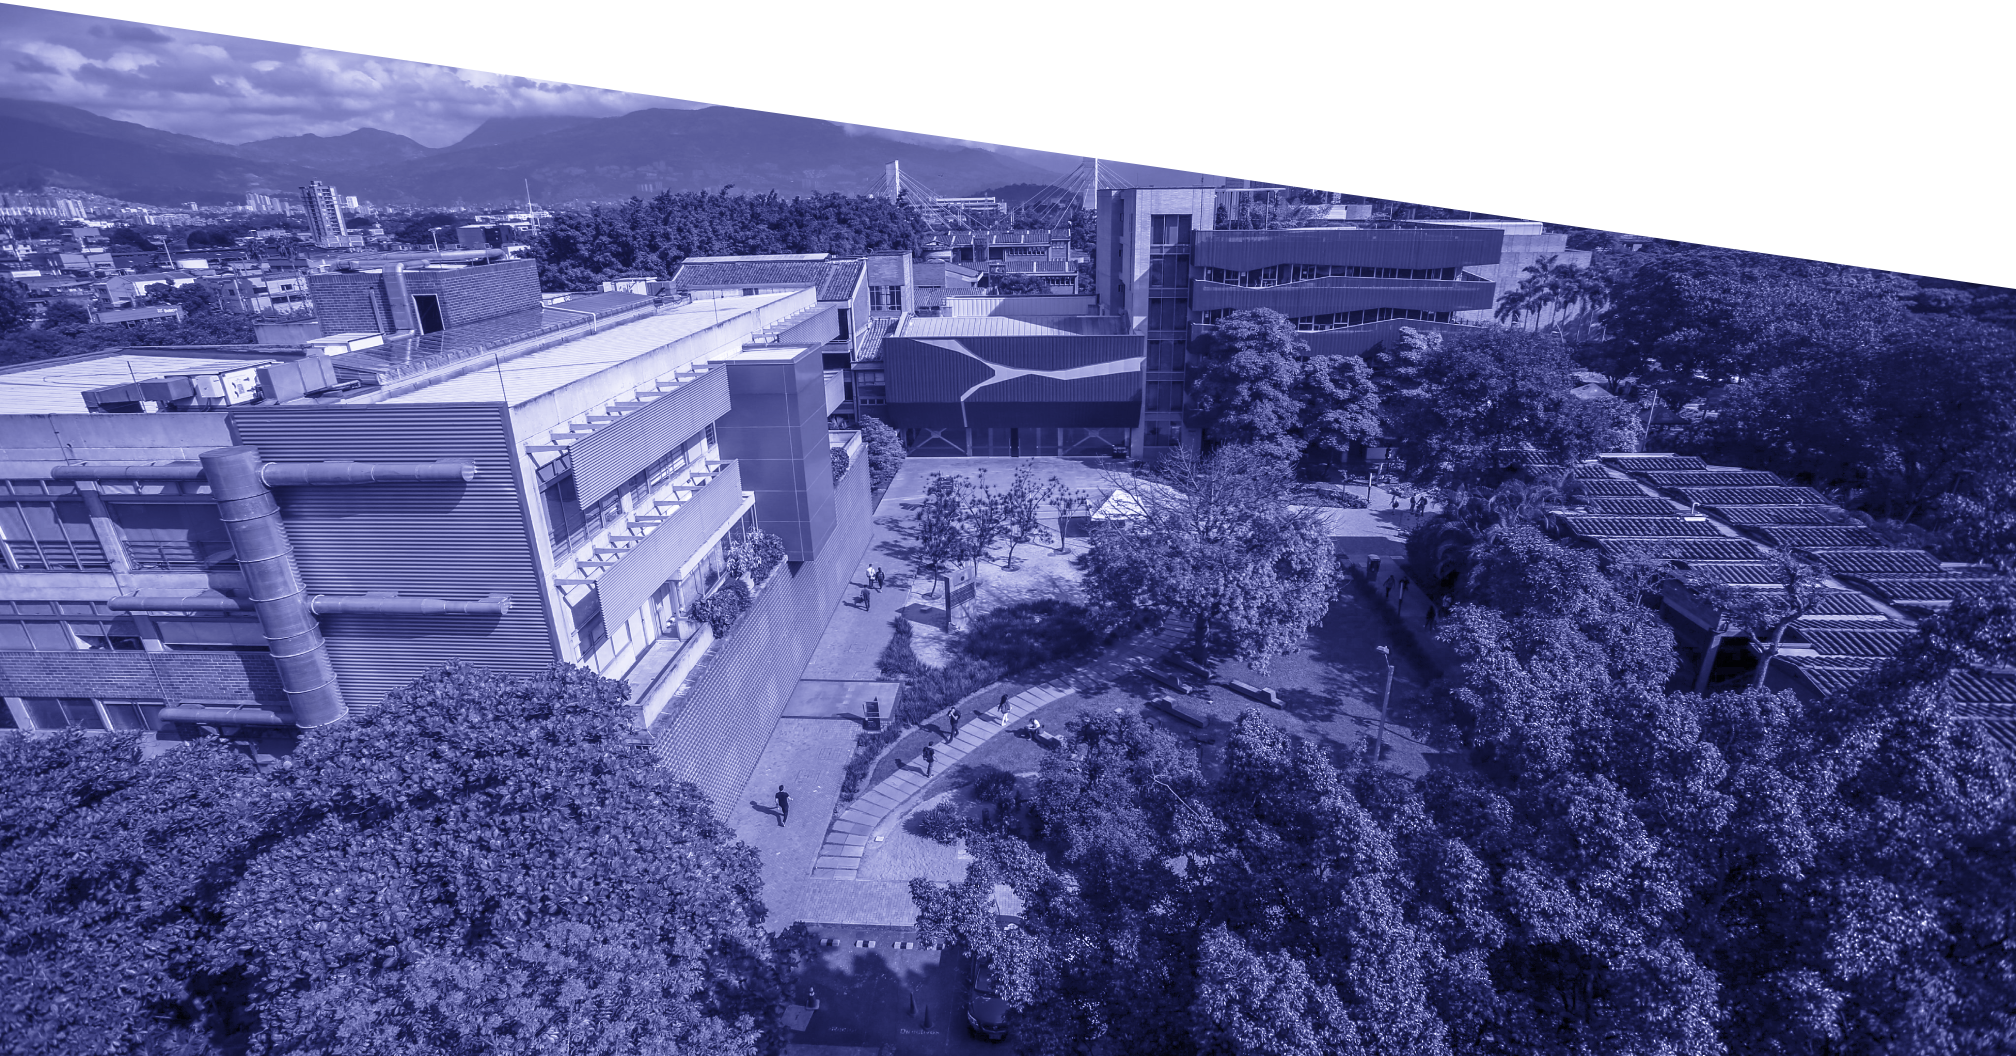
\includegraphics[width=\paperwidth]{Figures/0. General/eafit_banner.png}};

    \mbox{}
    \vfill
    \sffamily \Large \textcolor{white}{\placeanddate} \\



\end{titlepage}

\newpage

% Generates a ToC without page number
{
    \hypersetup{linkcolor=black} % Keeps the ToC black even with non-black linkcolor
    \tableofcontents
    \thispagestyle{empty}
}
\newpage

\section{Objetivo}

Desarrollar habilidades en la configuración, así como despliegue de aplicaciones
y servicios en red, particularmente las que requieren de una arquitectura
cliente/servidor.
\section{Problemática a resolver}

La empresa MiCompany S.A., requiere de un mecanismo basado en tecnologías de 
información (TI) que le permita capturar la opinión de los consumidores en
relación con los diferentes productos que tienen en el mercado.

En este sentido, le han solicitado a su empresa de soluciones de TI, que
implemente una estrategia que le permita recolectar lo que piensan los usuarios
de los productos. En la actualidad, la empresa cuenta con un catálogo de
cincuenta (50) productos. Básicamente, lo que se requiere es que el usuario
pueda expresar lo que piensa de uno o varios productos en particular, en no mas
de ciento cincuenta caracteres (150). Tenga en cuenta que, la única intención de
la empresa es que, posterior al proceso de recolección de datos, se pueda
aplicar técnicas de minería de texto sobre la información recolectada (p.ej, 
sentiment analysis, topic detection, etc) con el fin de extraer información de
cómo perciben los productos los clientes.

El director de TI de su empresa, ha decido para satisfacer la necesidad, implementar y 
desplegar una aplicación web para este proyecto. Al respecto, se ha definido que la 
aplicación debe contar con un proceso de registro de usuarios el cual captura: nombre, 
edad, ciudad, dirección, correo electrónico, entre otros datos relevantes (información 
sociodemográfica de los usuarios). De igual forma, la aplicación debe permitir la 
visualización de cada uno de los productos que tiene la compañía en el mercado y le debe 
permitir al usuario seleccionar el producto para que este pueda dar su opinión de este. 
Vale resaltar que un usuario, puede seleccionar uno o varios productos con el fin de dar 
su opinión de este.

Su área es la encargada de tanto del desarrollo como el despliegue de la aplicación web. 
Para esto se requiere que usted realice todo el proceso de diseño de la aplicación, la 
implementación, pruebas y puesta en producción de esta. Con respecto al proceso de 
despliegue, su empresa ha decidido que ésta se desplegada considerando una 
infraestructura de TI robusta y escalable para soportar la operación de la aplicación. Todo 
esto con el fin de garantizar como mínimo una disponibilidad de $99.5\%$. Tenga en cuenta 
que la aplicación debe desarrollarse que soporte de manera concurrente miles de
usuarios al igual que debe permitir escalar de manera horizontal.

En este sentido, desde la perspectiva del desarrollo de software a nivel de tecnologías, 
usted puede considerar cualquiera de los Manejadores de Contenido (CMS por sus siglas 
en inglés) disponibles en la actualidad (Drupal o Wordrpess), con el fin de desarrollar la 
aplicación para satisfacer la problemática planteada. Para efectos de la persistencia de 
datos, se debe considerar utilizar bases de datos propias que emplean este tipo de 
soluciones. 
Por otro lado, en los aspectos relacionados con el despliegue, se ha decidido que la 
aplicación web debe desplegarse utilizando un proveedor de computación en nube, 
utilizando el modelo de infraestructura como servicio (IasS). Tenga en cuenta que para 
desplegar la aplicación se requiere que usted considere elementos como balanceadores 
de carga para lograr un buen despliegue de la solución, de tal forma, que el balanceador 
de carga sea configurado para distribuir las peticiones entrantes entre diferentes 
servidores web que se tienen y los usuarios puedan tener acceso a la aplicación web 
desplegada. Es importante resaltar que, para acceder la aplicación usted debe tener un 
gestionar y conseguir un dominio público gratis de tal forma que la aplicación debe 
accederse a través de una URL, como, por ejemplo, \url{http://www.micompany.tk}. 
\section{Solución}

Como se mencionó anteriormente se espera \textbf{una escalabilidad horizontal} y
principalmente una \textbf{alta disponibilidad (99.5\%)}, además de esto el
cliente requiere de desplegarlo en \textit{AWS}. \\

Por lanto, de.
\newpage

% % Creates references using the Biblatex 
% \bibliographystyle{plain}
% \bibliography{General/References.bib}
% \newpage

% \appendix % Any section after this command will have a letter as an index

\end{document}
